% =========================================================================
% Capítulo 1: Cinemática
% Tema 03: Coordenadas intrínsecas
% Problema 04: Hélice y base intrínseca
% Origen: Ayudantía 5, 2026
% =========================================================================
\subsubsection{Hélice y base intrínseca}
Una partícula $P$ se mueve a lo largo de una hélice circular de radio $R$ y ángulo de inclinación constante $\phi$ respecto al plano horizontal, como se muestra en la Figura \ref{fig:c1_e03_p04_helice}. Determine:

\begin{enumerate}
    \item Los marcos de referencia y los sistemas de coordenadas.
    \item La velocidad y la aceleración de la partícula $P$.
    \item La base intrínseca $\{\vec{e}_t,\vec{e}_n,\vec{e}_b\}$.
\end{enumerate}

\begin{figure}[!ht]
    \centering
    \begin{tikzpicture}[>=Latex, x={(1cm,-0.2cm)}, y={(1cm,0.1cm)}, z={(0cm,1cm)}, scale=2]
        % --- Parámetros Geométricos ---
        \def\R{1.5}      % Radio
        \def\H{3.0}      % Altura
        \def\pitch{0.4}  % Paso de la hélice (proporcional a tan(phi))
        \def\pAng{120}   % Ángulo theta para la posición de P

        % --- 1. Ejes de Coordenadas ---
        \draw[->, thin, gray] (0,0,0) -- (2.5,0,0) node[right] {$x$};
        \draw[->, thin, gray] (0,0,0) -- (0,2.5,0) node[above right] {$y$};
        \draw[->, thick] (0,0,0) -- (0,0,3.5) node[above] {$z$};
        \node[below left] at (0,0,0) {$O$};

        % --- 2. Cilindro (Estructura) ---
        % Base inferior (parte trasera oculta)
        \draw[dashed, gray] (\R,0,0) arc (0:180:\R);
        % Base inferior (parte delantera)
        \draw[thick] (\R,0,0) arc (0:-180:\R);
        
        % Líneas laterales
        \draw[gray!50] (-\R,0,0) -- (-\R,0,\H);
        \draw[gray!50] (\R,0,0) -- (\R,0,\H);

        % Tapa superior (Elipse)
        \draw[thick, fill=gray!5, fill opacity=0.3] (0,0,\H) circle [radius=\R];

        % --- 3. Trayectoria Helicoidal ---
        % Hélice trasera (punteada)
        \draw[blue!50, dashed, domain=0:pi, samples=50, variable=\t] 
            plot ({\R*cos(\t r)}, {\R*sin(\t r)}, {\pitch*\t});
        \draw[blue!50, dashed, domain=2*pi:2.5*pi, samples=50, variable=\t] 
            plot ({\R*cos(\t r)}, {\R*sin(\t r)}, {\pitch*\t});

        % Hélice delantera (continua)
        \draw[ultra thick, blue!80!black, domain=pi:2*pi, samples=50, variable=\t] 
            plot ({\R*cos(\t r)}, {\R*sin(\t r)}, {\pitch*\t});
        \draw[ultra thick, blue!80!black, domain=-0.5*pi:0, samples=50, variable=\t] 
            plot ({\R*cos(\t r)}, {\R*sin(\t r)}, {\pitch*\t});

        % --- 4. Partícula P y Parámetros ---
        % Coordenadas de la partícula
        \pgfmathsetmacro{\Px}{\R*cos(\pAng)}
        \pgfmathsetmacro{\Py}{\R*sin(\pAng)}
        \pgfmathsetmacro{\Pz}{\pitch*\pAng*pi/180}
        
        \coordinate (P) at (\Px, \Py, \Pz);
        \coordinate (Pbase) at (\Px, \Py, 0);

        % Líneas de proyección
        \draw[dashed, thin] (0,0,0) -- (Pbase);
        \draw[dashed, thin] (Pbase) -- (P);
        \draw[dashed, thin] (P) -- (0,0,\Pz);

        % Partícula
        \filldraw[shading=ball, ball color=black] (P) circle (1.2pt) node[above right] {$P$};

        % Radio R y Ángulo Theta
        \draw[<->] (0,0,0) -- ({\R*cos(210)}, {\R*sin(210)}, 0) node[midway, below left] {$R$};
        \draw[->] (0.5,0,0) arc (0:\pAng:0.5);
        \node at (0.24, 0.32, 0) {$\theta$};

        % Ángulo de inclinación Phi
        \begin{scope}[shift={(1.5,0)}]
            \draw[dashed] (0,0,0) -- (0, 1.2, 0);
            \draw[->] (0, 0.4, 0) arc (20:90:0.4);
            \node[right] at (0.4, 0, 0.3) {$\phi$};
        \end{scope}


    \end{tikzpicture}
    
    \caption{Partícula $P$ en trayectoria helicoidal sobre un cilindro de radio $R$.}
    \label{fig:c1_e03_p04_helice}
\end{figure}

% --- SOLUCIÓN ---------------------------------------------------------------
\begin{solucion}{Hélice y base intrínseca}
\textbf{Marcos de referencia y Sistemas de Coordenadas}\\
Lo primero, como en todo ejercicio, es definir los marcos de referencia.
\begin{itemize}
    \item $\mathcal{N}$ El suelo $\longrightarrow\{\vec{E}_x;\vec{E}_y;\vec{E}_z\}$
    \item $\mathcal{A}$ Centro $O$ - proyección de $P$ $\longrightarrow\{\vec{e}_r;\vec{e}_\theta;\vec{e}_z\}$
\end{itemize}

\begin{center}
\begin{tikzpicture}[>=Stealth, scale=3]
    % --- SISTEMAS DE COORDENADAS ---
    \def\angOmega{55} % Ángulo de rotación
    \draw[->] (-1.2,0) -- (1.3,0);
    \draw[->] (0,-1.2) -- (0,1.3);
    \draw (0,0) circle (1);
    % Base fija (azul)
    \draw[->, blue, thick] (0,0) -- (0.8,0) node[anchor=north] {$\vec{E}_x$};
    \draw[->, blue, thick] (0,0) -- (0,0.8) node[anchor=east] {$\vec{E}_y$};
    % Base móvil (verde)
    \draw[->, green!60!black, thick] (0,0) -- (\angOmega:0.8) node[above left] {$\vec{e}_r$};
    \draw[->, green!60!black, thick] (0,0) -- (\angOmega+90:0.8) node[anchor=south east] {$\vec{e}_\theta$};
    % --- PUNTOS ---
    \fill[gray] (\angOmega:1) circle (2pt);
    \node[anchor=north west] at (\angOmega:1) {$P$};
    % --- ÁNGULO ---
    \draw (0.4,0) arc (0:\angOmega:0.4);
    \node at (25:0.5) {$\theta$};
    % Eje z saliendo de la página
    \draw[fill=white] (0,0) circle (0.08);
    \fill (0,0) circle (1pt);
    \node[anchor=north east] at (-0.05,-0.05) {$\vec{E}_z = \vec{e}_z$};
\end{tikzpicture}
\end{center}
\begin{equation*}
\begin{split}
    \vec{e}_r&=\cos(\theta)\vec{E}_x+\sin(\theta)\vec{E}_y\\
    \vec{e}_\theta&=-\sin(\theta)\vec{E}_x+\cos(\theta)\vec{E}_y\\
    \vec{e}_z&=\vec{E}_z
\end{split}
\end{equation*}

\subsubsection*{Cinemática de la partícula}
\textbf{Posición}\\
Como siempre, para obtener la velocidad de algún punto respecto a un marco de referencia inercial, hay que partir de la posición; en este caso la de la partícula $P$ es
$$\vec{r}_P=r\vec{e}_r+z\vec{e}_z$$
Y necesitamos encontrar $z$ en términos de cosas conocidas; para esto ocupamos el ángulo de inclinación $\phi$. Si nos vamos al borde del cilindro tenemos un triángulo en el cual el cateto inferior corresponde a la distancia recorrida en la dirección angular (también se puede ver diferencialmente como un pequeño cambio, la distancia recorrida es $Rd\theta$), que se puede representar como $R\theta$ donde recordemos que $\theta$ es el ángulo en radianes. Ahora nos falta el otro cateto, que corresponde a cuánto ha subido la partícula ($z$) respecto a cuánto se ha recorrido ($R\theta$).
\begin{center}
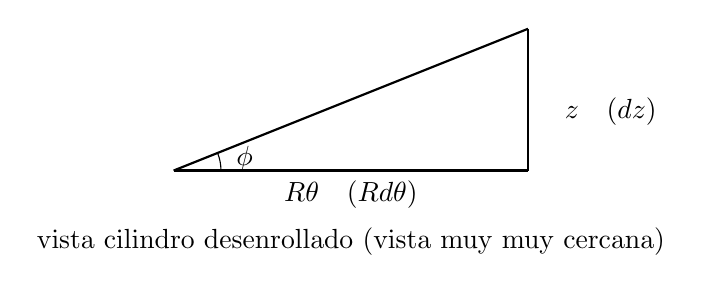
\begin{tikzpicture}[scale=1.5]
    % --- TRIÁNGULO (cilindro desenrollado) ---
    \draw[thick] (0,0) -- (3,1.2); % hipotenusa
    \draw[thick] (0,0) -- (3,0);   % base
    \draw[thick] (3,0) -- (3,1.2); % lado
    % --- ÁNGULO PHI ---
    \draw[dashed] (0,0) -- (0.8,0);
    \draw[dashed] (0,0) -- (0.8,0.32);
    \draw[-] (0.4,0) arc (0:21:0.4);
    \node at (0.6,0.1) {$\phi$};
    % --- ETIQUETAS ---
    \node at (1.5,-0.6) {vista cilindro desenrollado (vista muy muy cercana)};
    \node at (3.7,0.5) {$z\quad(dz)$};
    \node at (1.5,-0.2) {$R\theta \quad(Rd\theta)$};
\end{tikzpicture}
\end{center}
$$\tan(\phi)=\dfrac{z}{R\theta}=\dfrac{dz}{Rd\theta}\longrightarrow z=R\theta\tan(\phi)$$


\textbf{Velocidad}\\
Como se sabe, la velocidad es la derivada temporal de la posición desde un punto fijo.
$$\marc{\vec{v}_P}{N}=\der{\vec{r}_{P}}{N}=\der{(R\vec{e}_r+R)}{N}= R\der{\vec{e}_r}{N}+R\dot\theta\tan(\phi)\vec{e}_z$$
En este caso no es necesario utilizar teorema del transporte porque usamos el trucazo.\\
Derivadas temporales de $\vec{e}_r$ y $\vec{e}_\theta$
$$\transport{\vec{e}_r}{N}{A}=\dot\theta\vec{e}_z\times\vec{e}_r=\dot\theta\vec{e}_\theta $$
$$\transport{\vec{e}_\theta}{N}{A}=\dot\theta\vec{e}_z\times\vec{e}_\theta=-\dot\theta\vec{e}_r $$
y finalmente
$$\marc{\vec{v}_P}{N}=R\dot\theta\vec{e}_\theta+R\dot\theta\tan(\phi)\vec{e}_z$$

\textbf{Aceleración}\\
Al igual que antes podemos simplemente derivar la velocidad para obtener la aceleración.
$$\marc{\vec{a}_P}{N}=\der{\marc{\vec{v}_P}{N}{}}{N}{}=\der{\left(R\dot\theta\vec{e}_\theta+R\dot\theta\tan(\phi)\vec{e}_z\right)}{N}{}=(-R\dot\theta^2)\vec{e}_r+ R\ddot\theta\vec{e}_{\theta}+R\ddot\theta\tan(\phi)\vec{e}_z$$

\subsubsection*{Base intrínseca}
Para este caso la base intrínseca se define partiendo por el vector tangente
$$\vec{e}_t=\dfrac{\der{\vec{r}}{N}}{\left\|\der{\vec{r}}{N}\right\|}\quad\quad\quad\vec{e}_n=\dfrac{\der{\vec{e}_t}{N}}{\left\|\der{\vec{e}_t}{N}\right\|}\quad\quad\quad\vec{e}_{b}=\vec{e}_t\times\vec{e}_n$$
Entonces aplicando esto y calculando
$$\vec{e}_t=\dfrac{\der{\vec{r}_P}{N}}{\left\|\der{\vec{r}_P}{N}\right\|}=\dfrac{R\dot\theta(\vec{e}_\theta+\tan(\phi)\vec{e}_z)}{|R\dot\theta|\sqrt{1+\tan^2(\phi)}}=\dfrac{\vec{e}_\theta+\tan(\phi)\vec{e}_z}{\sqrt{1+\tan^2(\phi)}}$$
$$\vec{e}_n=\dfrac{\der{\vec{e}_t}{N}}{\left\|\der{\vec{e}_t}{N}\right\|}=\dfrac{\der{}{N}\dfrac{\vec{e}_\theta+\tan(\phi)\vec{e}_z}{\sqrt{1+\tan^2(\phi)}}}{\left\|\der{}{N}\dfrac{\vec{e}_\theta+\tan(\phi)\vec{e}_z}{\sqrt{1+\tan^2(\phi)}} \right\|}=-\vec{e}_r$$
$$\vec{e}_{b}=\vec{e}_t\times\vec{e}_n\longrightarrow\dfrac{\vec{e}_\theta+\tan(\phi)\vec{e}_z}{\sqrt{1+\tan^2(\phi)}}\times (-\vec{e}_r)=\dfrac{\vec{e}_z-\tan(\phi)\vec{e}_\theta}{\sqrt{1+\tan^2(\phi)}}$$

\textbf{Curvatura} (esto es extra)\\
La curvatura se define como la magnitud de la derivada del vector tangente sobre la velocidad, pero más que eso muestra cómo es que se curva este vector tangente, se asocia al inverso del radio que mejor describe esa curva.\\
En cálculo 3 se trabaja con longitud de arco, en este caso las trabajaremos con el tiempo
$$\kappa=\left\|\dfrac{d \,\vec{e}_t}{ds}\right\|=\left\|\dfrac{d \,\vec{e}_t}{dt}\dfrac{dt}{ds}\right\|\longrightarrow\left\|\dfrac{d \,\vec{e}_t}{dt}\dfrac{1}{\marc{}{N}v_P } \right\|$$
y podemos hacer lo mismo para el caso de la torsión $\tau$.
$$\tau=\left\|\dfrac{d \,\vec{e}_b}{ds}\right\|=\left\|\dfrac{d \,\vec{e}_b}{dt}\dfrac{dt}{ds}\right\|\longrightarrow\left\|\dfrac{d \,\vec{e}_b}{dt}\dfrac{1}{\marc{}{N}v_P } \right\|$$
Las derivadas de los vectores se pueden expresar como esta matriz
\[
\begin{pmatrix}
\frac{d\vec{e}_t}{dt}\\ \frac{d\vec{e}_n}{dt}\\\frac{d\vec{e}_b}{dt}
\end{pmatrix}
=
\|\marc{\vec{v}}{A}\|
\begin{pmatrix}
0 & \kappa & 0 \\
-\kappa & 0 & \tau \\
0 & -\tau & 0
\end{pmatrix}
\begin{pmatrix}
\vec{e}_t \\
\vec{e}_n \\
\vec{e}_b
\end{pmatrix}
\]

\patotruco{El ``trucazo'' de las cilíndricas: en lugar de aplicar el teorema del transporte, derivar la base directo con $\dfrac{d\vec{e}_r}{dt}=\dot\theta\,\vec{e}_\theta$ y $\dfrac{d\vec{e}_\theta}{dt}=-\dot\theta\,\vec{e}_r$. Esto funciona cuando $\vec{e}_\theta$ está definido en el sentido de $\theta$ creciente; si no, cambia el signo. Para esféricas conviene pasar a cilíndricas y usarlo ahí.}
\end{solucion}
